\documentclass[10pt,twocolumn]{article}

\usepackage[letterpaper,margin=0.56in]{geometry}
\usepackage{amsmath,amssymb,graphicx,booktabs,threeparttable,natbib,float,subcaption,placeins}
\usepackage[T1]{fontenc}
\usepackage[utf8]{inputenc}
\usepackage{lmodern}
\usepackage{caption}
\usepackage{hyperref}
\hypersetup{colorlinks=true, linkcolor=black, citecolor=blue, urlcolor=black}
\bibliographystyle{plainnat}
\setcitestyle{authoryear,round}
\captionsetup{font=scriptsize,labelfont=bf}
\captionsetup[subfigure]{font=scriptsize,skip=1pt}
\setlength{\floatsep}{4pt plus 1pt minus 1pt}
\setlength{\textfloatsep}{5pt plus 1pt minus 1pt}
\setlength{\dblfloatsep}{4pt plus 1pt minus 1pt}
\setlength{\dbltextfloatsep}{5pt plus 1pt minus 1pt}
\setcounter{topnumber}{4}
\setcounter{dbltopnumber}{4}
\renewcommand{\topfraction}{0.95}
\renewcommand{\dbltopfraction}{0.95}
\renewcommand{\textfraction}{0.03}
\renewcommand{\floatpagefraction}{0.85}
\renewcommand{\dblfloatpagefraction}{0.85}
\setlength{\parskip}{1pt}
\setlength{\parindent}{10pt}
\raggedbottom
\renewcommand{\abstractname}{Resumo}
\renewcommand{\refname}{Referências}
\renewcommand{\tablename}{Tabela}
\renewcommand{\figurename}{Figura}
\newcommand{\tabnotes}[1]{\par\vspace{2pt}\noindent\begin{minipage}{\linewidth}\footnotesize #1\end{minipage}}
\title{\vspace{-1.35cm}\textbf{Nota de Política Pública: saídas do Bolsa Família e emprego formal no município de Bento Gonçalves}}
\author{Victor Rangel\textsuperscript{*}\\[-1pt]{\normalsize Insper}}
\date{}

\begin{document}
\twocolumn[
\maketitle
\vspace{-0.55cm}
\begin{abstract}
\noindent Em novembro de 2024, o município de Bento Gonçalves iniciou uma política que combinou revisão cadastral do Bolsa Família, busca ativa de famílias em idade produtiva e encaminhamento a vagas formais. Esta nota estima seu efeito agregado com controle sintético. Em março de 2026, o município tinha 292 famílias a menos no programa do que seu contrafactual, e o estoque formal de empregos estava 496 vínculos acima da série sintética. Os resultados indicam que a queda de beneficiários veio acompanhada de melhora no mercado formal local, um padrão consistente com inclusão produtiva e relevante para decisões de escala e monitoramento.
\end{abstract}
\vspace{0.05cm}
\noindent{\footnotesize \textbf{Palavras-chave:} Bolsa Família; controle sintético; política municipal; emprego formal. \textbf{JEL:} I38; J68; C23; H53.}
\vspace{0.35cm}
]
\begingroup
\renewcommand{\thefootnote}{*}
\footnotetext{E-mail: \href{mailto:victorrsr@al.insper.edu.br}{victorrsr@al.insper.edu.br}. ORCID: \href{https://orcid.org/0000-0002-4520-2795}{https://orcid.org/0000-0002-4520-2795}.}
\endgroup

\section{Introdução}

Em novembro de 2024, o município de Bento Gonçalves passou a revisar o cadastro do Bolsa Família e encaminhar famílias em idade produtiva a vagas formais. A pergunta é se a queda subsequente de beneficiários excedeu a de municípios semelhantes e veio acompanhada de emprego formal. Sem essa segunda margem, a política poderia refletir correção cadastral ou perda de cobertura.

Esse é um problema de decisão pública. Indicadores próximos da regra de gestão podem responder sem garantir o desfecho social que justifica a política. Na proteção social, \citet{pradofirpo2026integridade} defendem batimentos de bases e revisão orientada por risco para fortalecer integridade e eficiência do gasto. Aqui, a dimensão adicional é emprego. A meta-análise de \citet{card2018what} mostra que políticas ativas de mercado de trabalho tendem a ter efeitos pequenos no curto prazo e mais positivos depois de dois ou três anos, com heterogeneidade por desenho e público atendido.

Transferências condicionadas podem afetar capital humano e trabalho. Avaliações do Bolsa Família encontram ganhos de escolaridade \citep{glewwe2012bolsa,debrauw2015schooling} e mobilidade posterior via saída de programas sociais e acesso ao emprego formal \citep{fassarella2024mobility}. Para o México, \citet{parker2023cct} mostram efeitos de longo prazo sobre escolaridade, mobilidade e mercado de trabalho. A evidência sobre oferta de trabalho é mais cautelosa do que a narrativa de desincentivo sugere \citep{debrauw2015labor,barbosa2014informality,banerjee2017lazy}. Estudos recentes também encontram maior duração no emprego formal e efeitos positivos de expansão de transferências sobre emprego \citep{santos2017duration,best2026productive}.

Estimo um controle sintético para o município de Bento Gonçalves usando municípios da região Sul. Os desfechos principais são famílias beneficiárias e estoque de vínculos formais. O segundo é agregado e não liga famílias individuais a postos de trabalho. Ainda assim, a série de emprego ajuda a separar inclusão produtiva de revisão administrativa.

\section{Estratégia empírica}

A estratégia segue o controle sintético de \citet{abadie2010synthetic}. A ideia é comparar o município tratado com uma média ponderada de municípios não tratados que reproduza sua trajetória antes da intervenção. O efeito mensal é $\alpha_{1t}=Y_{1t}-Y^N_{1t}$, em que $Y^N_{1t}$ é aproximado por $\widehat{Y}^N_{1t}=\sum_jw_jY_{jt}$, com $w_j\geq0$ e $\sum_jw_j=1$. Os pesos minimizam a distância pré-tratamento usando apenas informação anterior à intervenção.

Seleciono doadores antes de estimar os pesos. Restrinjo os candidatos a municípios completos e comparáveis no pool geográfico. Entre os candidatos mais próximos, escolho o subconjunto de 12 a 25 doadores que minimiza o RMSPE pré-tratamento do município de Bento Gonçalves. Bolsa Família usa todos os lags mensais disponíveis desde março de 2023. Estoque formal usa todos os lags desde fevereiro de 2023, mais log população e log PIB municipal. Nenhum resultado pós-tratamento participa da escolha.

O pool principal é a região Sul (RS, SC e PR). A Tabela~\ref{tab:results} também mostra uma especificação restrita ao Rio Grande do Sul. O tratamento operacional é novembro de 2024. As figuras usam média móvel de 3 meses. Os $p$-valores reportados são os testes de efeito nulo derivados da rotina SCM.CS de \citet{firpo2018synthetic}. As bandas mostram seus conjuntos de confiança de 90\%. Os dados combinam MDS/VISDATA, Novo CAGED e covariáveis municipais da Base dos Dados.

\begin{table*}[t]
\centering
\caption{Estimativas de controle sintético para Bolsa Família e emprego formal}
\label{tab:results}
\begin{threeparttable}
\small
\setlength{\tabcolsep}{5pt}
\begin{tabular*}{\linewidth}{@{\extracolsep{\fill}}l c r r r r r@{}}
\toprule
Desfecho & Pool & Doadores & RMSPE pré & Pós/pré & $p$ & Efeito final \\
\midrule
Bolsa Família (famílias) & Sul & 12 & 2.11 & 6.21 & 0.077 & -292\textsuperscript{*} \\
 & RS & 12 & 2.06 & 6.56 & 0.077 & -312\textsuperscript{*} \\
Estoque formal (vínculos) & Sul & 20 & 0.43 & 3.76 & 0.056 & 496\textsuperscript{*} \\
 & RS & 20 & 0.45 & 3.23 & 0.312 & 559 \\
\bottomrule
\end{tabular*}
\tabnotes{\textit{Notas:} A tabela reporta os desfechos destacados no texto principal, em suas unidades indicadas. Doadores é o número de municípios retidos na especificação escolhida pelo ajuste pré-tratamento. Os $p$-valores placebo excluem doadores cujo MSPE pré-intervenção é mais de cinco vezes maior que o MSPE pré-intervenção do município de Bento Gonçalves. Estrelas no efeito final indicam \textsuperscript{*}$p<0{,}10$, \textsuperscript{**}$p<0{,}05$ e \textsuperscript{***}$p<0{,}01$.}
\end{threeparttable}

\end{table*}

\begin{figure*}[t]
\centering
\makebox[\textwidth][c]{%
\begin{minipage}{0.995\textwidth}
\centering
\subcaptionbox{Bolsa Família: Observado e sintético}[0.486\textwidth]{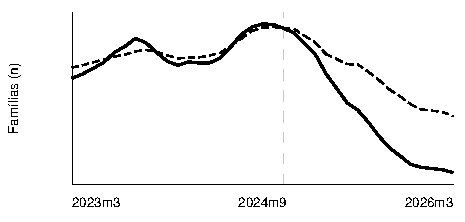
\includegraphics[width=0.486\textwidth]{figures/fig_main_01_bolsa_familia_series.pdf}}\hspace{0.006\textwidth}%
\subcaptionbox{Estoque formal: Observado e sintético}[0.486\textwidth]{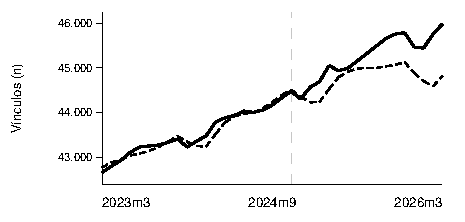
\includegraphics[width=0.486\textwidth]{figures/fig_main_02_emprego_estoque_series.pdf}}

\vspace{2pt}
\subcaptionbox{Bolsa Família: Gap e IC 90\%}[0.486\textwidth]{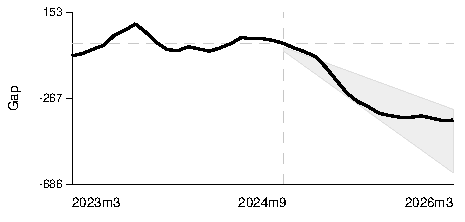
\includegraphics[width=0.486\textwidth]{figures/fig_main_01_bolsa_familia_ci.pdf}}\hspace{0.006\textwidth}%
\subcaptionbox{Estoque formal: Gap e IC 90\%}[0.486\textwidth]{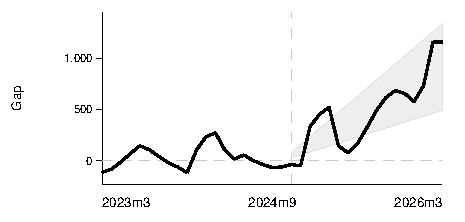
\includegraphics[width=0.486\textwidth]{figures/fig_main_02_emprego_estoque_ci.pdf}}

\vspace{2pt}
\subcaptionbox{Bolsa Família: Placebos}[0.486\textwidth]{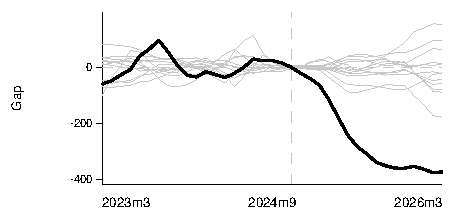
\includegraphics[width=0.486\textwidth]{figures/fig_main_01_bolsa_familia_placebo.pdf}}\hspace{0.006\textwidth}%
\subcaptionbox{Estoque formal: Placebos}[0.486\textwidth]{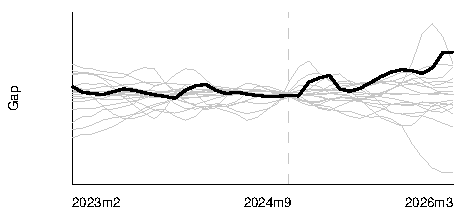
\includegraphics[width=0.486\textwidth]{figures/fig_main_02_emprego_estoque_placebo.pdf}}
\end{minipage}%
}
\caption{Controle sintético, pool Sul. Painéis à esquerda reportam famílias beneficiárias. Painéis à direita reportam estoque de vínculos formais. Séries em média móvel de 3 meses. No último mês, o efeito é -292 famílias no Bolsa Família ($p_{FP}=0.077$) e 496 vínculos no estoque formal ($p_{FP}=0.048$).}
\label{fig:main-att}

\par\vspace{1pt}
\begin{minipage}{0.96\textwidth}
\footnotesize\emph{Principais pesos do pool sintético. Bolsa Família tem 12 municípios com peso positivo, liderados por Esperança do Sul/RS 9.0\%, Cruz Alta/RS 8.5\%, Santa Vitória do Palmar/RS 8.5\%. Estoque formal tem 20 municípios com peso positivo, liderados por Sant'Ana do Livramento/RS 5.0\%, Santa Maria/RS 5.0\%, Ijuí/RS 5.0\%.}
\end{minipage}

\end{figure*}


\FloatBarrier
\vspace{5pt}
\section{Resultados}

Os painéis comparam o município de Bento Gonçalves ao seu contrafactual sintético nos dois desfechos centrais. O Bolsa Família cai 292 famílias no último mês ($p_{FP}=0.077$). O estoque formal fica 496 vínculos acima do sintético ($p_{FP}=0.048$). Esse segundo resultado é compatível com maior inserção no mercado formal local no período posterior à política.

A queda no Bolsa Família equivale a 18\% do município sintético em março de 2026. O efeito no estoque formal é menor em termos proporcionais, cerca de 1\%, mas soma 496 vínculos. Isso corresponde a 1,7 vínculo formal para cada família a menos no programa no último mês. Na média pós-tratamento, a razão é próxima de 2,1 vínculos por família. A comparação sugere magnitudes administrativamente próximas, embora a série agregada não permita concluir que as famílias que saíram foram exatamente as contratadas.

O exercício principal retém os doadores com melhor desempenho pré-tratamento dentro do pool regional. São 12 municípios para Bolsa Família e 20 para estoque formal. Essa seleção melhora o ajuste visual no pré-tratamento e evita um pool amplo demais para uma aplicação municipal.

A leitura causal deve permanecer no nível agregado. A trajetória do município de Bento Gonçalves se afasta do contrafactual regional, o que enfraquece uma leitura puramente descritiva de queda mecânica no Bolsa Família. O mecanismo permanece em aberto. O aumento de estoque formal é consistente com inclusão produtiva, mas dados individuais são necessários para verificar se as famílias que saíram do programa foram absorvidas pelo mercado formal.

\section{Considerações finais}

Depois de novembro de 2024, o município de Bento Gonçalves registra menos famílias no Bolsa Família e mais vínculos formais do que seria esperado a partir de municípios semelhantes da região Sul. O contrafactual sintético disciplina a comparação e reduz o risco de confundir a política local com movimentos regionais comuns. A leitura mais prudente é que há evidência consistente de queda adicional no Bolsa Família e sinal compatível de melhora no mercado formal local. O desenho não identifica quem saiu do programa.

Os resultados sustentam monitoramento e investigação. Adoção em outros municípios deveria depender de replicação local, persistência dos efeitos e validação individual do mecanismo. A próxima etapa é ligar Cadastro Único, folha de pagamentos do programa, RAIS/CAGED e trajetórias de renda. Esses dados permitiriam verificar se as famílias que saíram do programa foram absorvidas pelo mercado formal, em quais ocupações, com que salários e por quanto tempo. Se o mecanismo for confirmado, a experiência oferece uma hipótese concreta de política municipal a ser adaptada em outros contextos. Até lá, políticas que afetam renda, trabalho e acesso a direitos devem ser avaliadas com contrafactuais claros e comunicadas com incerteza.

\newpage
\setlength{\bibsep}{0pt plus 0.1ex}
\bibliography{references}

\clearpage
\onecolumn
\appendix
\section*{Apêndice A. Informações de submissão}
\setlength{\parindent}{0pt}
\setlength{\parskip}{4pt}

\textbf{Título em inglês (English title)}

Public Policy Note: Bolsa Família exits and formal employment in the municipality of Bento Gonçalves.

\section*{Abstract}

In November 2024, the municipality of Bento Gonçalves launched a policy combining Bolsa Família registry review, outreach to working-age families, and referrals to formal jobs. This note estimates its aggregate effect with synthetic control. In March 2026, the municipality had 292 fewer families in the program than its counterfactual, and formal employment stood 496 jobs above the synthetic series. The results indicate that beneficiary exits were accompanied by improvement in the local formal labor market, a pattern consistent with productive inclusion and relevant for scale-up and monitoring decisions.

\textbf{Palavras-chave em inglês (Keywords)}

Bolsa Família; synthetic control; municipal policy; formal employment.

\textbf{ORCID}

Victor Rangel: \href{https://orcid.org/0000-0002-4520-2795}{https://orcid.org/0000-0002-4520-2795}.

\textbf{Declaração de contribuição dos autores}

Este manuscrito é de autoria única. A declaração de contribuição dos autores não se aplica.

\textbf{Conflito de interesses (Conflict of interest)}

O autor declara não haver conflito de interesses financeiro, institucional ou pessoal relacionado a este manuscrito.

\textbf{Declaração de disponibilidade de dados de pesquisa (Data availability statement)}

O código, a base final usada nas estimativas principais e as instruções de reprodução estão disponíveis em \url{https://github.com/vr-rodrigues/bento-goncalves-bolsa-familia-synth}. Os dados brutos são provenientes de bases públicas e podem ser regenerados pelos scripts e consultas SQL do projeto.

\textbf{Dados e uso de IA}

Este projeto utilizou IA agentic, via Codex, como apoio à pesquisa, com organização do projeto, coleta e checagem de dados, refinamento de código, geração de tabelas e rotinas de reprodutibilidade. A pergunta, as escolhas econométricas, a interpretação substantiva e a responsabilidade por eventuais erros são integralmente do autor.

\end{document}
